\documentclass{article}
\usepackage{float}
\usepackage{graphicx}
\newcommand{\popcnt}{\texttt{\_\_builtin\_popcount }}
\linespread{1.2}
\begin{document}
\title{600.639 Computational Genomics\\
Final Project}
\date{}
\author{Ashleigh Thomas and Jed Estep}
\maketitle

\begin{abstract}
Easily searchable representations of genome strings are useful for many kinds of analysis, but in practice their usability is often limited on commodity hardware due to their high memory requirements. Suffix arrays are one of the least memory-intensive commonly used representations, but its space requirements may still be prohibitive in the case of indexing numerous genomes. In this paper we investigate the suffix array compression scheme described in \cite{GV05}. We attempt to apply the compressed suffix arrays as a searchable database of multiple genomes with use in the context of metagenomics. The design of our database is similar to that of QUASAR \cite{B99}.
\end{abstract}
\section{Introduction}
\label{sec-intro}
\indent We arrived at this design while investigating multiple topics. From one end, we were interested in pursuing the applicability of compressed data structures to representing genomes. Many implementations of useful index structures like suffix trees are extremely memory intensive, so decreasing the size of their representation is paramount if they are to be used on commodity hardware. Literature on the topic of succinct data structures often neglects to discuss practical versions of their structures, and as such we explore how well the methods of \cite{GV05} work in a real program.\\
\indent From an alternative angle, we noted that most approaches to metagenomics rely on probabilistic methods, such as \cite{BS09}, and less attention is given to index search methods that are commonly used for read alignment. We wanted to explore the usefulness of string indexing in identifying the source of a read from an unknown genome. We operate under the following assumption: at least some reads from a particular random sample of DNA will come from one lone source, provided that the reads are short enough. In other words, the kind of DNA collected in metagenomics is not totally fragmented, but stays in clumps of some unknown length $k$. As long as we are searching for $q$-grams such that $q < k$, we should be able to identify some sources of a read using exact or approximate matching.\\

\section{Prior Work}
\label{sec-prior-work}
Burkhardt \cite{B99} points out that, in the operation of QUASAR, numerous special methods are necessary to accommodate suffix arrays which are too large to fit in main memory. As such, we attempted to apply the compression methods of Grossi and Vitter \cite{GV05} to a search index similar to QUASAR. The compressed suffix array implementation of our choice has a few notable properties:
\begin{enumerate}
\item In comparison to compressed representations of permutations \cite{BN08}, it has a much faster time for random access, which is vitally important for our desired application, and
\item Its implementation has not been explored in any major public implementation, such as the SDSL library \cite{SDSL}.
\end{enumerate}
While \cite{GV05} proposes a novel structure and retrieval algorithm for its suffix array, the primary technique of compression (decreasing the size of an array $\Psi$, whose definition is discussed both in \cite{GV05} and section ~\ref{subsec-sa}) can be swapped out for a more standard one for compressing vectors of integers, such as the methods of \cite{E75}.

\section{Methods and Software}
\label{sec-methods-software}
\subsection{Suffix Arrays}
\label{subsec-sa}
We implemented both a compressed and uncompressed suffix array representation, as well as a database that stores labels and genomes and can be queried with reads.\\
\indent The uncompressed suffix array is implemented as an array of integers. The actual substrings are not saved in the class. In addition to standard functionality, each suffix array has the ability to create an array $B$. $B$ is defined as follows \cite{GV05}:
\begin{figure}[H]
$B[i] = SA[i]\;\%\;2$
\end{figure}
\indent We are able to represent $B$ as a simple \texttt{unsigned char\*} with each value being a single bit. Not only is this representation highly compact, but we obtain several useful properties, particularly in the computation of $rank(B,i)$. Using the SSE4.2 extension to the x86 architecture, we can compute the rank on 4-byte chunks using the \popcnt function. This saves space over the original description, which used a rank-select dictionary to store $rank$ explicitly.\\
\indent The implementation of the compressed suffix array extends suffix array. Added class variables include the number of levels $k$, which is the maximum number of times the suffix array can be compressed; a vector of arrays $B_i$ for $0 < i < k$, which we refer to as the \emph{odd-even arrays}; and a vector of arrays $\Psi_i$, which we refer to as the \emph{companion arrays}. $\Psi$ is defined as follows \cite{GV05}:
\begin{figure}[H]
\label{fig-defn-psi}
$\Psi[i] = i$ if $SA[i]\;\%\; 2 = 0$\\
$\Psi[i] = j$ where $SA[j] = SA[i]+1$ otherwise
\end{figure}
Additionally, a lookup method is implemented based on \cite{GV05} with several small modifications; we describe the need for these in Section~\ref{sec-conclusions}.\\
\begin{figure}[H]
\label{fig-csa-repr}
\caption{\small\small\textit{All information produced after a single level of compression. Figure courtesy of \cite{GV05}.}}
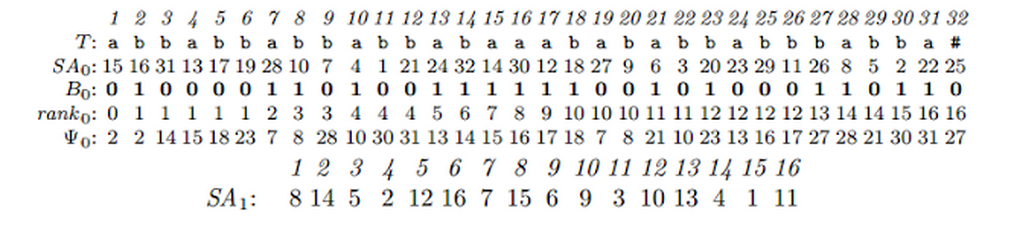
\includegraphics[width=12cm]{csa.png}\\
\end{figure}
\indent Each array $\Psi_i$ is implemented as a standalone class, holding a reference to the array $B_i$ and an integer array, which is a cache of the values represented by $\Psi_i$, and which we will call \texttt{values}. While \cite{GV05} describes a succinct method for representing \texttt{values}, we chose to investigate a different approach. The paper mentions defining \texttt{values} as a total function, i.e. it contains the mapped value for every valid input. In practice, this is not necessary, as $\Psi_i[j] = j$ whenever $B_i[j] = 1$. Therefore, we store only half the possible values of $\Psi_i$ in \texttt{values}, specifically those for which $B_i[j] = 0$. While only half the values in the codomain of $\Psi_i$ are stored explicitly, storing them directly led to an increase in overall size of the data structure when compared to a standard suffix array. As such, we stored them in a compressed integer array from the SDSL-Lite library implementation by Simon Gog \cite{SDSL}. This vector class first encodes its integers as their deltas, then applies a self-delimiting code to the result. \cite{OS07}.\\
\indent We made overall a number of decisions in this implementation which differed from the initial report substantially. These decisions were made in the context of ignoring theoretical bounds in places where they were not meaningful, in favor of building a real, practical implementation. The first major change is that $rank$ is not represented explicitly at all. Each time we compute $rank(i)$, we perform an $O(|B_i|)$ calculation, which seems drastically unimproved from the constant bound proposed in the paper. But in reality, the \popcnt instruction operates with incredible speed; computing the rank of a 100 million byte array took around 220ms. Thus, while the theoretical bound of lookup is increased, the practical speed is not seriously impacted and no extra bits are used to store $rank$.\\
\indent We also tried multiple algorithms for building the uncompressed suffix array, which is a requirement for building a compressed suffix array. Our initial algorithm uses a sorted hashmap with key-value pairs \texttt{std::<string, int>}, holding a substring and its index. Once built, the suffix array is the list of values. Using the C++ class \texttt{std::map}, which has $O(\log n)$ inserts in general but amortized constant, we got a worst case bound for the build time of $O(n\log n)$. However, the map requires $O(n^2)$ space; while this is all freed once the array is built, it can be prohibitive on larger string inputs. We also used a more common method of sorting the strings in length-based blocks, increasing by a power of 2 each time. This approach runs in $O(n \log^2 n)$ and uses $O(n)$ extra memory. While we hoped that this method would run faster due to not requiring memory paging, in practice both implementations had impractically long build times for large strings. As such, our tests were run on smaller data, using the former $O(n\log n)$ method of construction.
\subsection{Database}
\label{subsec-db}
\indent There is an implementation of a class that represents an entry in the database, called a \emph{genome entry}. This consists of a label (the name of the species that the genome is from), the genome, and the associated compressed suffix array of this genome.\\
\indent Finally, we implement the database in a straightforward manner as a \texttt{std::vector} of genome entries. Users can query the database with strings and receive the labels of the genomes that the read is contained in within the database. The database holds a vector of genome entries. The primary query API is the function \texttt{getGenomeLabel(const string\&)}. This method calls a basic binary search on each genome entry in the database, which searches through the genome to find the correct index if one exists. When landing on long substrings, the binary search checks if the input read is a prefix of the substring; this leads our binary search to be $O(n \log m)$ (where $n = |genome|$ and $m = |input|$) in the worst case, though in practice it is often faster than that as most suffixes are much shorter than $n$.\\

\section{Results}
\label{sec-results}
We have produced significant compression in our implementation. We ran our implementation on a randomly generated read of 60,000 nucleotides. The suffix array took up 240,048 bytes, while the compressed suffix array took up 106,998 bytes. This is a compression of 56\%. There is a time performance penalty in constructing the compressed suffix array; while the uncompressed version built in 281ms, the compressed version built in 1352ms. We found that indexing performance on the two of them was nearly identical.\\
\indent While the above results suggest that build times are reasonable, we found that for strings of a length appropriate for an assembled chromosome, the time required to build even an uncompressed suffix array was not practical (at least on \texttt{ugrad12}). Not only did this bottleneck prevent us from testing on large datasets, as even after 15 minutes or more the suffix arrays were still building, but it revealed an important underlying assumption of \cite{GV05}: that a complete, uncompressed suffix array is always available. For the purpose of a database, which will be computing the compressed suffix arrays only once (and, in a more sophisticated implementation, caching them on disk when possible), it still precludes the idea of using the compressed suffix array on commodity hardware. Even if the amount of RAM required to store the compressed array is small enough to be practical for an average computer, the uncompressed suffix array still needs to be built and stored in RAM as an intermediate result. This diminishes the usefulness of a compressed suffix array for an application of this kind.
\section{Conclusions}
\label{sec-conclusions}
While we have made significant improvements on the space that a suffix array takes up, there are several key points to consider about this implementation.\\
\indent First, it is important to note that the method described by Grossi and Vitter actually increases the size of the suffix array, unless the array $\Psi$ is bit-compressed (using either their method or another). Therefore the size of the compressed suffix array becomes larger than that of the original suffix array. This is repaired by using the \texttt{enc\_vector} encoding \cite{E75, SDSL}. This utilizes deltas in order to compress the compressed suffix array further, contributing to the 56\% compression.\\
\indent Grossi and Vitter use one-indexed arrays in their algorithm. This brings up a few problems, as the algorithm will work in only two cases. The first is that the arrays are one-indexed and the genome string is of even length. This is because if we are using a one-indexed array and an odd length genome, the largest index of the suffix array is odd but has no companion. This breaks the calculation of $\Psi$. The second case is when the arrays are zero-indexed and the genome string is of odd length. In \cite{GV05}, the authors explore building compressed suffix arrays on strings whose length is a power of 2, and do not appear to consider the case of odd length strings. While it is easy in theory to ignore this case, in practice it is unreasonable to assume all input strings have even length.\\
\indent Although the explored method is both efficient in practical search applications once built and offers substantial data compression, we feel overall that the method is not necessarily practical. The construction of an initial suffix array may be prohibitive in its running time if the suffix array is to be built on commodity hardware; in the case of running on a computing cluster, it is not clear that compression is especially necessary for holding multiple structures concurrently in RAM.
\clearpage
\begin{thebibliography}{1}
\bibitem{GV05}
	Roberto Grossi and Jeffrey Vitter,
	\emph{Compressed Suffix Arrays and Suffix Trees with Applications to Text Indexing and String Matching}.
	Society for Industrial and Applied Mathematics Journal of Computing,
	Vol. 35, No. 2, pp. 378-407,
	2005.
\bibitem{B99}
	Stefan Burkhardt, et al.,
	\emph{q-gram Based Database Searching Using a Suffix Array (QUASAR)}.
	Proceedings of the third annual international conference on Computational molecular biology,
	pp. 77-83,
	1999.
\bibitem{BS09}
	Arthur Brady and Steven Salzberg,
	\emph{Phymm and PhymmBL: Metagenomic Phylogenetic Classification with Interpolated Markov Models}.
	Nature Methods,
	2009.
\bibitem{OS07}
	Daisuke Okanohara and Kunihiko Sadakane,
	\emph{Practical Entropy-Compressed Rank/Select Dictionary}. 
	Proceedings of the 9th Workshop on Algorithm Engineering and Experiments,
	ALENEX,
	2007.
\bibitem{E75}
	Peter Elias,
	\emph{Universal Codeword Sets and Representation of the Integers}.
	IEEE Transactions on Information Theory,
	Vol. 21, No. 2,
	1975.
\bibitem{BN08}
	Jeremy Barbay and Gonzalo Navarro,
	\emph{Compressed Representations of Permutations, and Applications}.
	Technical Report TD/DCC-2008-18,
	University of Chile,
	2008.
\bibitem{SDSL}
	Simon Gog,
	\emph{Succinct Data Structures Library lite}.
	https://github.com/simongog/sdsl-lite,
	2008.
\bibitem{CF11}
	---,
	\emph{Suffix Arrays}.
	http://codeforces.com/blog/entry/4025,
	2011.
\end{thebibliography}
\end{document}